\section{Load and Priority Based Consistent Hashing} % Based Load Balancing Policies}
\label{sec:chrlu}

In this section, we describe the load-balancing algorithm that takes into consideration function locality and priority, bursty workloads, and stale server load information. 
We assume a cluster of homogeneous servers, and that a new function invocation can be sent to any of the servers.
Each server implements keep-alive for functions: after successful execution, the function's container is stored in server memory, and evicted based on some eviction policy.

\begin{figure}
\centering
  \hspace{-1.5cm}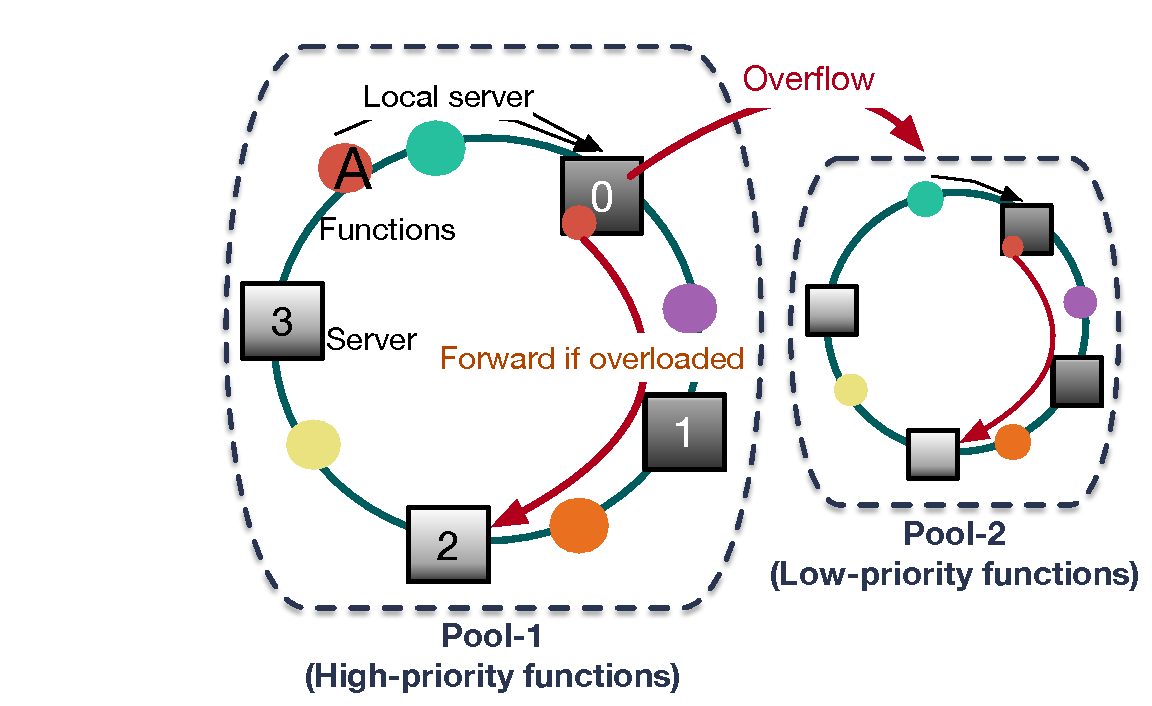
\includegraphics[width=0.48\textwidth]{../figs/k-rlu2.pdf}
  \caption{$k$-CH-RLU partitions a cluster into multiple server pools and runs server-load-aware consistent hashing in each pool. Functions are forwarded if servers are overloaded, or to a lower-priority pool if the entire pool is.}
  \label{fig:2-pool-arch}
\end{figure}

% Overview of the architecture. 
\noindent \textbf{Architecture.}
To support QoS for functions of different priority levels, we use a two-stage load-balancing architecture (see Figure~\ref{fig:2-pool-arch}). 
The cluster is partitioned into multiple pools, one for each priority level.
For ease of exposition and without loss of generality, we consider two levels: high- and low-priority functions, and thus two corresponding pools. 
Within a single pool, functions are load-balanced among servers using a load-aware consistent hashing technique. 
Our approach is modular: each pool runs an independent load-balancing policy, which is the focus of most of this section. 
This approach also preserves function locality, which is important for reducing cold-starts, as we describe next.  

%This two-stage architecture is modular: we can run different load-balancing policies within each pool. % This can come later. Subtle but important point. 



% such as LRU, TTL, or Greedy-Dual~\cite{faascache-asplos21}. 
%Subsequent invocations of the function constitute  a ``warm'' start which is significantly faster than a cold start. 
%The keep-alive policy determines when and which functions to evict when the server memory is fully occupied by running and ``warm'' containers.

% Thus, locality is crucial for achieving low latency.
% Data storage clusters such as distributed key-value stores also require object-access requests to be routed to the same set of servers.
% However, locality is a stronger constraint in data storage because of consistency requirements. 
% In the case of functions, locality is preferable, and server loads are also considered. 

% Where is the queueing theory perspective? LWL/ SJF/ dispatch. Highly variable job lengths.
%\vspace*{-0.2cm}
\subsection{Tradeoff between Locality and Load}
\label{subsec:locality-load-xoff}
We use consistent hashing as the fundamental principle to ensure high locality: repeated invocations of the same function occur on the same server. 
However, popular functions, i.e., which are invoked very frequently, can result in overloaded servers.
Because function performance is affected by server load and resource availability, focusing on locality alone can result in slow function execution.

Function popularities are also highly skewed: a small percentage account for a vast majority of invocations.
With pure locality-based load-balancing, the servers of these popular functions would be severely overloaded.
Functions also can run for significantly longer than simple web requests, and thus they impose more load on servers, and the cost of a wrong placement decision is higher. 
This, combined with bursty invocations, can significantly increase the tail latency of functions. 
Thus, pure-locality policies such as classical consistent hashing are not sufficient, and 
our research question is: \emph{Can consistent hashing be used to reduce latency due to overloaded servers?} 
Or put another way, can we balance the tradeoff between function locality and server loads with consistent hashing? 
%
Our key idea is to extend consistent hashing to take also into account server loads, the cold-start overheads of different functions, and the bursty traffic that is a key characteristic of FaaS workloads.
%In the rest of this section, we describe our approach. 

% \subsection{Broad design Criteria}
% LB latency is important: millisecond pricing, so LB cant take up too many cycles.

%\vspace*{-0.2cm}
\subsection{Key Principle: Load-based Forwarding}
\label{subsec:key-principle}

To balance the locality vs. server load tradeoff, we build on a new variant of consistent hashing called Consistent Hashing with Bounded Loads~\cite{mirrokni2018consistent} (abbreviated as CH-BL in the rest of the paper).  
The key idea behind CH-BL is to use consistent hashing to locate servers for objects, and if the servers are ``full'', then ``forward'' the objects to the next server in the consistent hashing ring.

For example, in Figure~\ref{fig:ch}, function A is originally assigned to server 0, but this ``home'' server is overloaded (already running many functions), and thus the function is forwarded along the ring until a suitable non-overloaded server (2) is found. 
Any 5-independent hashing function can be used for determining the ``home'' server of a function. %which is determined by hashing the function's unique id. 
Users can specify the load upperbound or the capacity of the server ($b$), which determines the max load the server can sustain.  
Consistent hashing with bounded loads provides many strong theoretical guarantees on the length of the forwarding chain until the object is safely placed on a server. 

Interestingly, forwarding along the ring not only avoids server overload, but also improves locality, \emph{even in overload scenarios}.
Forwarding along the ring has the advantage that even if a function is not run on its ``home'' server, subsequent invocations that ``overflow'' still have a high warm-start probability on the servers in the overflow chain. %, with the warm-start probability decreasing in chain-length.
The warm-start probability is highest on the home server, and decays the farther the function is from it. 
This works better than alternative techniques such as Consistent Hashing with Random Jumps~\cite{chrj-aaai21}, which do not preserve locality and forwards to a randomly chosen least loaded server. 

%\vspace*{-0.2cm}
\noindent \textbf{Server Load}
is a key metric in load-balancing policies to  determine the \emph{relative} suitability of one server over another.
OpenWhisk currently uses occupied-memory used by active/running invocations as a proxy for load, and is unsuitable because functions have highly variable CPU utilization. 
%
Instead, we primarily rely on \emph{system-level} load metrics, such as the standard Linux 1-minute load-average, which captures CPU utilization and 
I/O wait due to cold-starts, and provides a more realistic measure of load.
%Traditional Linux load-average estimates the total number of processes running and ready-to-run, and
We normalize the load-average by the number of CPUs. 
Thus, a load-average of $8$ on an 8 core server (discounting hyperthreading) is normalized to 1. 
%
An important practical consideration is that load information is often \emph{stale} due to delays in monitoring and collection, with the degree of staleness ranging from a few seconds to several minutes.
Techniques for ameliorating the staleness are presented in Section~\ref{subsec:random-stale-loads}. 
%For instance, because the Linux load average is an exponential moving average, it is slow to change.
%Furthermore, load monitoring and reporting has delays due to how frequently the metrics are gathered at the local server, and how often they are made available to the load-balancer.
%We use a simple publish-subscribe-like system, where individual servers periodically (every 5 seconds) push their load information, and the load-balancer uses these published loads to make all scheduling decisions.


%\subsection{Cold-Start Aware Bounded-Loads

%\vspace*{-0.2cm} % Challenges of CH-BL adoption.
\begin{comment}
\subsection{Why CH-BL Is Insufficient}

The high computing load of functions, their bursty nature, and the staleness of loads, are the three major challenges to Consistent Hashing with Bounded Loads~\cite{mirrokni2018consistent} that the original algorithm is not designed to meet. 
There are a few practical considerations and key differences between simple object/storage caching and function execution:
1. CH-BL does not take into account the heterogeneity in running times and memory size of the objects (i.e., functions).
2. The implicit CH-BL performance model is binary: running-time is assumed to be uniform as long as servers are under the load-bound. 
3. The server loads evolve as a result of the actual function execution and are not just uniformly incremented as in the original algorithm. Object deletions are also not handled explicitly: we let the lazily computed load average determine whether a server meets the load-bound or not. 

\emph{Importantly, we do not assume complete and consistent state information about the servers.}
Omniscient knowledge of the execution state of all functions running all servers can certainly be leveraged effectively to run functions on the most suitable server.
However, such maintaining such global knowledge is expensive and impractical as far as storage consistency and latency are concerned.
Thus, we are striving for load-balancing policies which are robust to stale, incomplete, and coarse-grained information about server states. 
In the rest of this section, we shall show how the above three limitations of CH-BL can be overcome in FaaS load-balancing settings. 
\end{comment]

%\vspace*{-0.4cm}
\subsection{Incorporating Function Performance Characteristics}
\label{subsec:chch}


Different running time and performance characteristics of functions can be incorporated into consistent hashing.
\emph{The key problem is to determine when and which function to forward.}
The forwarding policies need to be cognizant of the warm and cold running times, and the sensitivity to load of different functions. 

%Each server has a load-bound which we do not want the server's load to exceed. As described in the previously, consistent hashing with bounded loads can ensure that no individual server exceeds the load-bound $c$, by forwarding the request (in our case, function invocation) to the next server in the ring, until a suitable server is found. This bound determines what the maximum load of the servers will be. 


Assume a load-bound of $b$, the warm time of a function is $w$, and the cold time is $c$ (slow-start). 
%
The current or the home server will be ``0'', and the next server in the ring that the function may be forwarded-to will be denoted by ``1''. 
Running it on the ``home''/local server will result in expected time $E[T_0] = (p_0w+(1-p_0c)S(L_0) $, where $p_0$ is the cache-hit/keep-alive probability, and $S(L_0)$ is the slowdown in function if the load on the server is $L_0$. 
When a function in invoked the load balancer has the choice to either run in on the home server or forward it to the next server, where it is less likely to be found in the keep-alive cache, because the reuse-distance is much larger for the servers down the chain.
Therefore we can compute the forwarding regret, $E[T_0]/E[T_1]$.

The properties of bounded-loads allows us to easily compute this value.
The probability of being forwarded is small, and is $1/b$ based on Lemma 4 of~\cite{mirrokni2018consistent}.
The reuse-distance of the function, and hence the hit-rate on the original/home server will be larger: $p_0 > p_1*b$. 
Based on our empirical observation of sub-linear performance decrease due to load (Section~\ref{subsec:function-perf}), in the worst case, the home server will be overloaded and alternative server will not be, and hence the ratio of slowdowns, $S(L_0)/S(L_1) > b$.
%
Minimizing the regret, we get that the function should be forwarded if $L>cb/w$.
Thus, the effective load upper-bound is \emph{increased} by a factor of $\text{cold}/\text{warm}$  time, allowing us to run more functions per server. 
In our empirical evaluation, we will show that this can significantly improve performance over plain CH-BL with a function-agnostic constant load-bound.
If the cold and warm times of a function are not available, then they are assumed to be equal, thus this degrades to classic function-agnostic bounded-loads. 


%%%%%%%%%%%%%%%%%%%%%%%%%%%%%%%%%%%%%%%%%%%%%%%%%%%%%%%%%%%%

%\vspace*{-0.4cm}
\subsection{Handling Bursts}
\label{subsec:bursty}

Functions come in a variety of frequency classes and are also prone to unpredictable burstiness (i.e., very low inter-arrival-times for a short duration). 
Identifying these bursts and both keeping latency for such ``popular'' functions low and preventing them from negatively impacting co-located functions is critical.
We have found that handling overload conditions is a key requirement and can significantly affect the tail latency.

Bursty function invocations result in two main problems.
First, they cause an increase in server load beyond the actual load-bound, because load is only lazily tracked.
The delayed load information can result in a popular function completely overwhelming a server, causing load ``hotspots'' in the cluster.
The second problem is that in extreme cases, the inter-arrival-time is less than the function latency, causing concurrent invocations.
Even if these concurrent invocations are run on a ``local'' server with the function present in the keep-alive cache, there will still be cold-starts, since each invocation must run in its own container. 

Our solution to these two problems caused by bursty invocations is to detect popular function bursts, ``spread'' these invocations around multiple servers to prevent cluster hot-spots, and use stochastic/random load updates to introduce randomness into the load-balancing. 

\begin{comment}
Multiple problems. 1. Increase the load beyond the bound because lazily tracked. 2. Concurrent: no warm starts. Spreading them around will be useful. 

The problem of concurrent invocations is vexing even with locality, since containers may be in use and thus results in cold-starts for these invocations. In the worst case we must accept $n-1$ cold starts for an $n$ core server. 

% Very popular functions can present problems.
We use two strategies:
1. Identify popular functions in a low-overhead online manner.
1a. Use this information to inform the load estimate. Due to the problem of \textbf{stale loads.}
2. Extreme overload: pick least loaded server if going around the horn.  % this seems orthogonal. 

This is similar to epsilon-greedy: we greedily pick the server based on the expected running time estimate for unpopular functions and probabilistically for popular functions. 
The probability is determined based on the server load and the noise in the server load estimate, which in turn depends on the estimate of the recent arrival rate of the functions. 

\end{comment}

%\vspace*{-0.2cm}
\subsubsection{Detecting Popular Functions with Spatial Sampling}

Our goal is to detect ``popular'' functions with low inter-arrival times, in an online low-overhead manner.
%
Popularity detection must take into account the changing invocation frequencies of different functions over time, and be low-overhead.
We identify the top \textit{p} percentile of functions by their inter-arrival times (IAT), or below some explicit IAT threshold, to reduce unnecessary hyperparamaters. 

Our approach is general: we build a histogram of inter-arrival times using sampling and then query it. 
We note similarities with computing reuse distance histograms, which are the building block of miss-ratio curves. 
%Our goal is to find the popular functions that have a low inter-arrival-time (IAT) quickly.
Reuse time histograms are a simpler version of reuse distances:
Reuse distance is the number of \emph{unique} objects accessed, whereas inter-arrival time is the difference in wall-clock times.
%In particular, we use the SHARDS technique, and modify and simplify it to compute an approximate IAT distribution instead of a reuse distance distribution. 



Our solution to identifying popular functions and function bursts is inspired by the popular SHARDS~\cite{shards} algorithm for building reuse distance histograms. 
%
Following SHARDS, we randomly sample invocations to track individual function IATs. 
This tracking is simplified by only recording the most recent access time, and then computing the IAT as an estimated moving average of the current IAT and  $now - last\_access$. 
These values are tracked for every function, and functions in the top $p^{th}$ percentile of IATs are considered \textbf{popular}.
%
For the sampled functions using spatial hashing, we update their IAT.
Note that this approach keeps only a small number of last-accessed IAT entries in memory: ``have-been'' popular functions are naturally evicted from the tracking list. 
Since we do not care about reuse distances, we avoid keeping a tree of reuse distances, resulting in a simplified SHARDS-like algorithm (see Algorithm~\ref{algo:shards-popular}). 


% \begin{lstlisting}
% def update_shards_popular(func, time):

% if Ti < T:
%   if func in last_access_times:
%     # Already in our sample set 
%     iat = (t-last_access_times[func])/R 
%     last_access_times[func] = t 
%     prev_iat = iat_dict[func]
%     iat_dict[func] = iat 
%     iat_heap.remove((prev_iat, func))
%     iat_heap.push((iat, func))
%   else:
%     #First access... iat=='inf'
%     last_access_times[func] = t 
%     iat_dict[func] = t/R 
%     iat_heap.push((t/R, func))
%   iats_only = [x[0] for x in h]
%   pop_thresh = percentile(iats_only, 20)
%   avg_iat = percentile(iats_only, 50)
%   avg_arrival_rate = 1.0/(1000.0*avg_iat)
% \end{lstlisting}

\begin{algorithm}
% \begin{algorithmic}
\caption{SHARDS-inspired popular function detection. Functions with the top p percentile of IATs are `popular'.}
\begin{algorithmic}[1]

  \Procedure{update\_shards\_popular}{$func, time$}
 \State $P \gets 100.0$
 \State $T \gets 20.0$ 
 \Comment{Effective sampling rate}
 \State $R \gets T / P$ 
 \State $Ti \gets abs(hash(func.name))$ 
 \If{$Ti \leq T$}
  \If{$last\_access\_times.contains(func)$}
  \Comment{Already in our sample set} 
  \State $iat \gets (t-last\_access\_times[func])/R$
  \State $last\_access\_times[func] = t$ 
%  \State $prev\_iat = iat\_dict[func]$
%  \State $iat\_dict[func] = iat$
%  \State $iat\_heap.remove((prev\_iat, func))$
  \State $iat\_heap.push((iat, func))$
  \Else
  \Comment{First access... iat=='inf'}
  \State $last\_access\_times[func] = t$
%  \State $iat\_dict[func] = t/R$
  \State $iat\_heap.push((t/R, func))$
  \EndIf
 \EndIf
 \State $iats\_only \gets iat\_heap.values()$
 \State $pop\_thresh \gets percentile(iats\_only, p)$
% \State $avg\_iat \gets percentile(iats\_only, 50)$
%  \State $avg\_arrival\_rate \gets 1.0/(1000.0*avg\_iat)$
\EndProcedure
\end{algorithmic}
\label{algo:shards-popular}
\end{algorithm}

%\vspace*{-0.2cm}
\subsubsection{Randomly Updating Stale Loads}
\label{subsec:random-stale-loads}

Popular functions represent such a large percentage of invocations yet a small number of functions that they can be safely spread across multiple servers without causing cold starts.
A fair load balancing algorithm must spread popular functions to ensure QoS for less frequent functions. 
As load information is stale, enforcing locality and load can result in servers facing a herd effect.
Randomization is a powerful strategy to ameliorate this; but, we must use it judiciously due to the strong effects on locality in FaaS load balancing.

Our solution is to introduce random forwarding (along the ring) proportional to the load of the server, such that popular functions are forwarded with a higher probability. 
If the (stale) load of the server is $L$, we update its load by adding gaussian noise with a mean of the \emph{extra anticipated load} on the server, based on the staleness and server-level function arrival rate ($\lambda$).
Specifically, $L_{\text{noisy}}=L+\mathcal{N}(\mu=\lambda, \sigma=0.1)$, where $\mathcal{N}$ is a Gaussian random variable. 
For popular functions, we  compare the $L_{\text{noisy}}$ to the load bound.
For remaining functions, we continue to use the stale load $L$. 
Thus, for highly loaded servers ``near'' the upper bound, the extra random noise will result in the popular bursty functions being forwarded more to avoid the herd effect.

\begin{comment}
To achieve this, we introduce Gaussian noise to the forwarding decision.
% is added to the load based on the iat and the rate. Per-function noise. Can also be just a per-server estimate if desired. 
We compute the global arrival rate, then estimate the per-server arrival rate and the effect an invocation has on server load, following the steps in Algorithm~\ref{algo:PopularRLUPolicy}.
For each server we then sample noise from the normal distribution whos mean is centered on the \textit{extra\_anticip\_load}, and add that to the server's tracked load to get \textit{Lnoise}.
We iterate along the ring of servers until we find one with a \textit{Lnoise} less than the global \textit{bounded\_ceil}.
In the case where we skip over 3 servers, we assume that the invocation will run cold no matter what, and assign it to the least loaded server.
\end{comment}

% \textbf{Question 1:} Why not do the stale load error correction for all functions, why just the popular ones?

\subsection{Putting it all Together: $k$-CH-RLU}
\label{subsec:chrlu}

Our overall policy, Consistent Hashing with Random Load and Updates with $k$ pools ($k$-CH-RLU), combines all the previously described techniques and insights.

Upon a new function invocation, it runs in its pool using the \texttt{forward} procedure in Algorithm~\ref{algo:PopularRLUPolicy}, which combines the use of SHARDS for popularity detection, cold and warm times for increasing the effective load bound, and noisy loads. 
The initial server is determined using a consistent hashing function. 
We bound the cold/warm ratio with a final load upper bound, $b\_max$.
The load-bound parameters determine the locality sensitivity: higher values of $b$ and $b\_max$ increase locality at the risk of resource-contention delays.
Similarly, higher values of $p$ results in more aggressive random forwarding and reduces locality. 

Our two-level architecture is modular and allows us to parameterize different load-balancing policies for different pools.
Lower-priority pools are run with a higher load bound $b\_max$, and thus tolerate more overloaded servers, at the risk of lower function performance.
Forwarding along the chain has diminishing returns on locality, and if the function gets forwarded more than $max\_chain\_len$ times, it triggers the overflow condition.

Function prioritization and QoS are controlled via the server pools: Each function has a default pool based on their priority level, with higher-priority functions having lower pool numbers. 
The high-priority functions recursively overflow to the next lower-priority pool, and thus have good locality because all pools use our consistent hashing approach. 
The high-priority functions can thus overflow and potentially use the entire cluster in case of workload spikes, preserving their QoS. 
The lower-priority pools thus also serve as a ``burst buffer,'' crucial considering the bursty nature of functions. 
Low-priority functions can't make use of higher-priority servers even if they are available, since we want to be able to handle bursty invocations of higher-priority functions. 
For the lowest-priority pool, we run the function on the least-loaded server in their pool. 
%
If the least loaded server is also overloaded, we drop the function.
% \begin{figure}
\begin{algorithm}[t]
  \caption{$k$-CH-RLU}
  \begin{algorithmic}[1]
    \Procedure{forward}{$pool, func, server, chain\_len $}
    \State $b, b\_max, max\_chain\_len \gets system\_params $
    \If{$ chain\_len > max\_chain\_len $} \Comment Overflow 
    \If{$ pool == k $} \Comment Lowest-priority pool
    return least-loaded-server
    \Else \State forward(pool+1, func, server=CH(func, pool), 0) \Comment Try in next pool 
    \EndIf 
    \EndIf 

    \State $\lambda \gets 1.0 / avg\_iat$ \Comment Computed from Algo 1
     \State $L=Load(server)$
    \If{popular(func)} \Comment Computed from Algo 1 
         \State $L = Load(server) + \mathcal{N}(\mu=\lambda\,\sigma=0.1)$
    \EndIf 
    \If{$L < min(cb/w, b\_max)$}
       \State server
\Else \State forward(pool, func, next(server), chain\_len+1)
       \EndIf
       \EndProcedure
    \end{algorithmic}
\label{algo:PopularRLUPolicy}
\end{algorithm}

% \begin{algorithm}
  
% \end{algorithm}



\noindent \textbf{Pool Sizing.}
The priority pools are sized proportional to the number of functions registered at different priority levels.
Thus, if 25\% of all functions are low-priority, then 25\% of the servers are in the low-priority pool and the rest are in the high-priority pool.
Periodically, we recompute this ratio based on the currently registered functions, which may lead to resizing the pools.
Importantly, locality is preserved even after pool resizing because of consistent hashing. 


\begin{comment}
We have also implemented a simple PID controller with hysteresis for horizontal scaling, by using server load averages as the input control signal. 
This horizontal scaling is conservative, with a large dead-band of 5 minutes, and scaling is triggered only if the at least 50\% of the servers are overloaded.
As we shall show in the empirical evaluation, CH-RLU significantly reduces the variance in the loads among servers, and thus is more amenable to this horizontal scaling policy. 
\end{comment}


% Unpopular functions still use Algorithm~\ref{algo:ConsistentCachePolicy}.
% In all cases, if we exhaust the list of servers trying to find one with low load, we randomly assign the invocation to a server.
% This only occurs in the most extreme cases of system load and also prevents spamming a popular server in that same scenario.



% if popular: L+Noise > bound 
% else: L > bound 

%%% Local Variables:
%%% mode: latex
%%% TeX-master: "paper"
%%% End:
